\chapter{Background: WebAssembly {\&} WebAssembly System Interface}
This chapter gives insight in what \acrfull{Wasm} is and how it works, alongside additional insight in how the \acrfull{WASI} works and how it is progressing.

\section{\acrshort{Wasm}}

When the web was born, the only supported programming language supported on the web was Javascript. As a relatively simple and portable language this did suffice. Over the years the web has become more complex and has become the center of the personal computer. However, its supported technologies did not grow at the same expansion pace. Javascript is still the only supported language and hampers the further expansion of the web. New technologies have been created to fix this issue, but none have succeeded. 
In order to be a viable Javascript alternative, a new model needs to be safe, fast, portable and compact. \acrshort{Wasm} is the first new technology to check all these four boxes. \cite{bringing_the_web_up_to_speed}

\subsection{Safe}
Wasm is intended to run in various environments, with some executing Wasm code from unknown sources. The web is a prime example of such a case. In these cases, it is required that the code runs in a sandbox, so that it cannot access all resources of the device. This way, malicious code can only do harm in the sandbox, and not the entire device.

Additionally, a Wasm program is often build in multiple modules. A Wasm module can be seen as an island of code, which imports and exports functions. Each module has its own stack, memory, types and more. This means that each module is isolated and cannot affect other modules, increasing the security of the model. Additionally, Wasm makes use of a linear memory model (Figure \ref{fig:wasm_high_level}). Each module gets its own range, and can only access that part of the memory.

\subsection{Portable}
\acrfull{Wasm} works as a compilation target for programming languages. Languages can compile to Wasm, just like they would for e.g. x86.
To compile to Wasm, the source code is first compiled to an intermediate representation, such as the LLVM IR. This is universal and also happens when compiling to other architectures. This part of the compilation process, called the frontend, stays the same. The backend of the compilation process, where the code gets translated into machine instructions, differs per instruction set. In the backend of the compiler the code will get compiled to the Wasm instruction set and output Wasm bytecode. This binary can get executed by a Wasm runtime. (Figure \ref{fig:wasm_compiler_frontend}) The bytecode is platform-agnostic, so it can run on any hardware and operating system that has a Wasm runtime. This makes Wasm portable.

This general idea works great for compiled languages, such as C, Rust or Swift. However, for interpreted languages such as Python, the model will work different. On native instruction sets, interpreted languages are read at runtime by their interpreter, which is often written in C. To make this work in Wasm, the interpreter can be compiled to Wasm and can interpret the language source code, just like it would happen on a native machine.

\subsection{Compact}
To achieve a small program, which is often critical for quickly loading websites, Wasm acts as a stack machine instead of a register-based machine. In register-based machines, registers are used to make calculations. On stack machines, argument values and operands are pushed on the stack, and result values are popped from the stack (Figure \ref{fig:wasm_high_level}). \cite{bringing_the_web_up_to_speed} By not having the need for registers, the binary size can be made smaller. \cite{stack_vs_register_machine} Another advantage of this method is that the amount of available registers can vary on different platforms. This is not an issue with stack machines.

\begin{figure}[h]
  \centering
  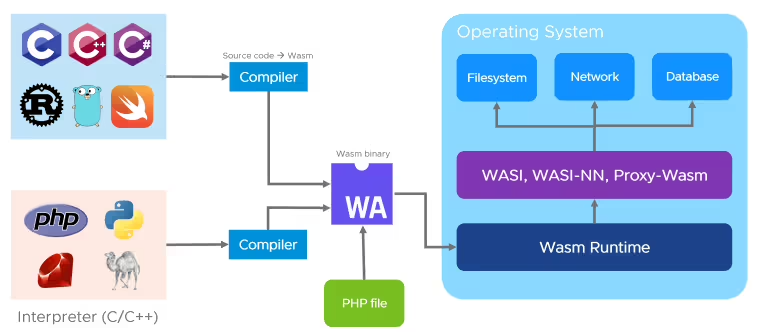
\includegraphics[width=1\textwidth]{images/wasm_compiler.png}
  \caption{Source code gets compiled to the Wasm architecture. The Wasm runtime executes the Wasm bytecode. \cite{docker_without_containers}}
  \label{fig:wasm_compiler_frontend}
\end{figure}

\begin{figure}[h]
  \centering
  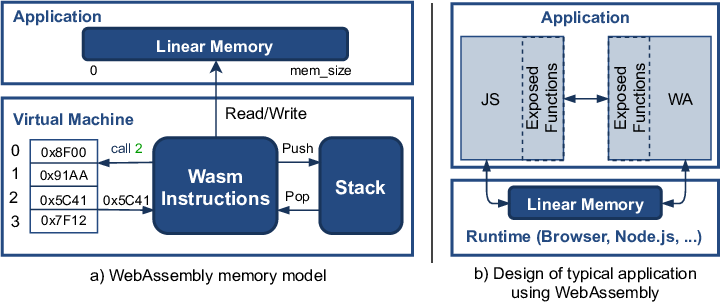
\includegraphics[width=1\textwidth]{images/WebAssembly-high-level-architecture.png}
  \caption{Wasm internals \cite{wasm_vulnerabilities}}
  \label{fig:wasm_high_level}
\end{figure}

\section{\acrshort{WASI}}

When writing code that compiles to Wasm, there is a need for system interfaces. These are required to do useful stuff, such as getting access to files. In the browser, WebAssembly applications can use Javascript as a system interface. However, outside the browser, there is no such predefined system interface. To solve this problem the \acrfull{WASI} was created. \acrshort{WASI} is a set of portable APIs, similar to APIs you would find in an operating system.

\subsection{The Component Model}

\subsection{\acrshort{WIT}}

\subsection{Milestones}

